%%%%% Single page layout:
%%%%% ----------------------------------------------------
\documentclass[12pt, a4paper]{report}
\usepackage{preamblePackage}
\usepackage{code}
%%%%%%%%%%%%%%%%    DOCUMENT    %%%%%%%%%%%%%%%%%%%%%%%%%%%%%%%%    DOCUMENT    %%%%%%%%%%%%%%%%%%%%
% \setcounter{secnumdepth}{-1} % sections are level 1
\begin{document}
%UVODNA CAST
% \frontmatter %first pages of the document


\subfile{title.tex}

\savegeometry{g}

\newgeometry{offset = 5mm}
\newpage
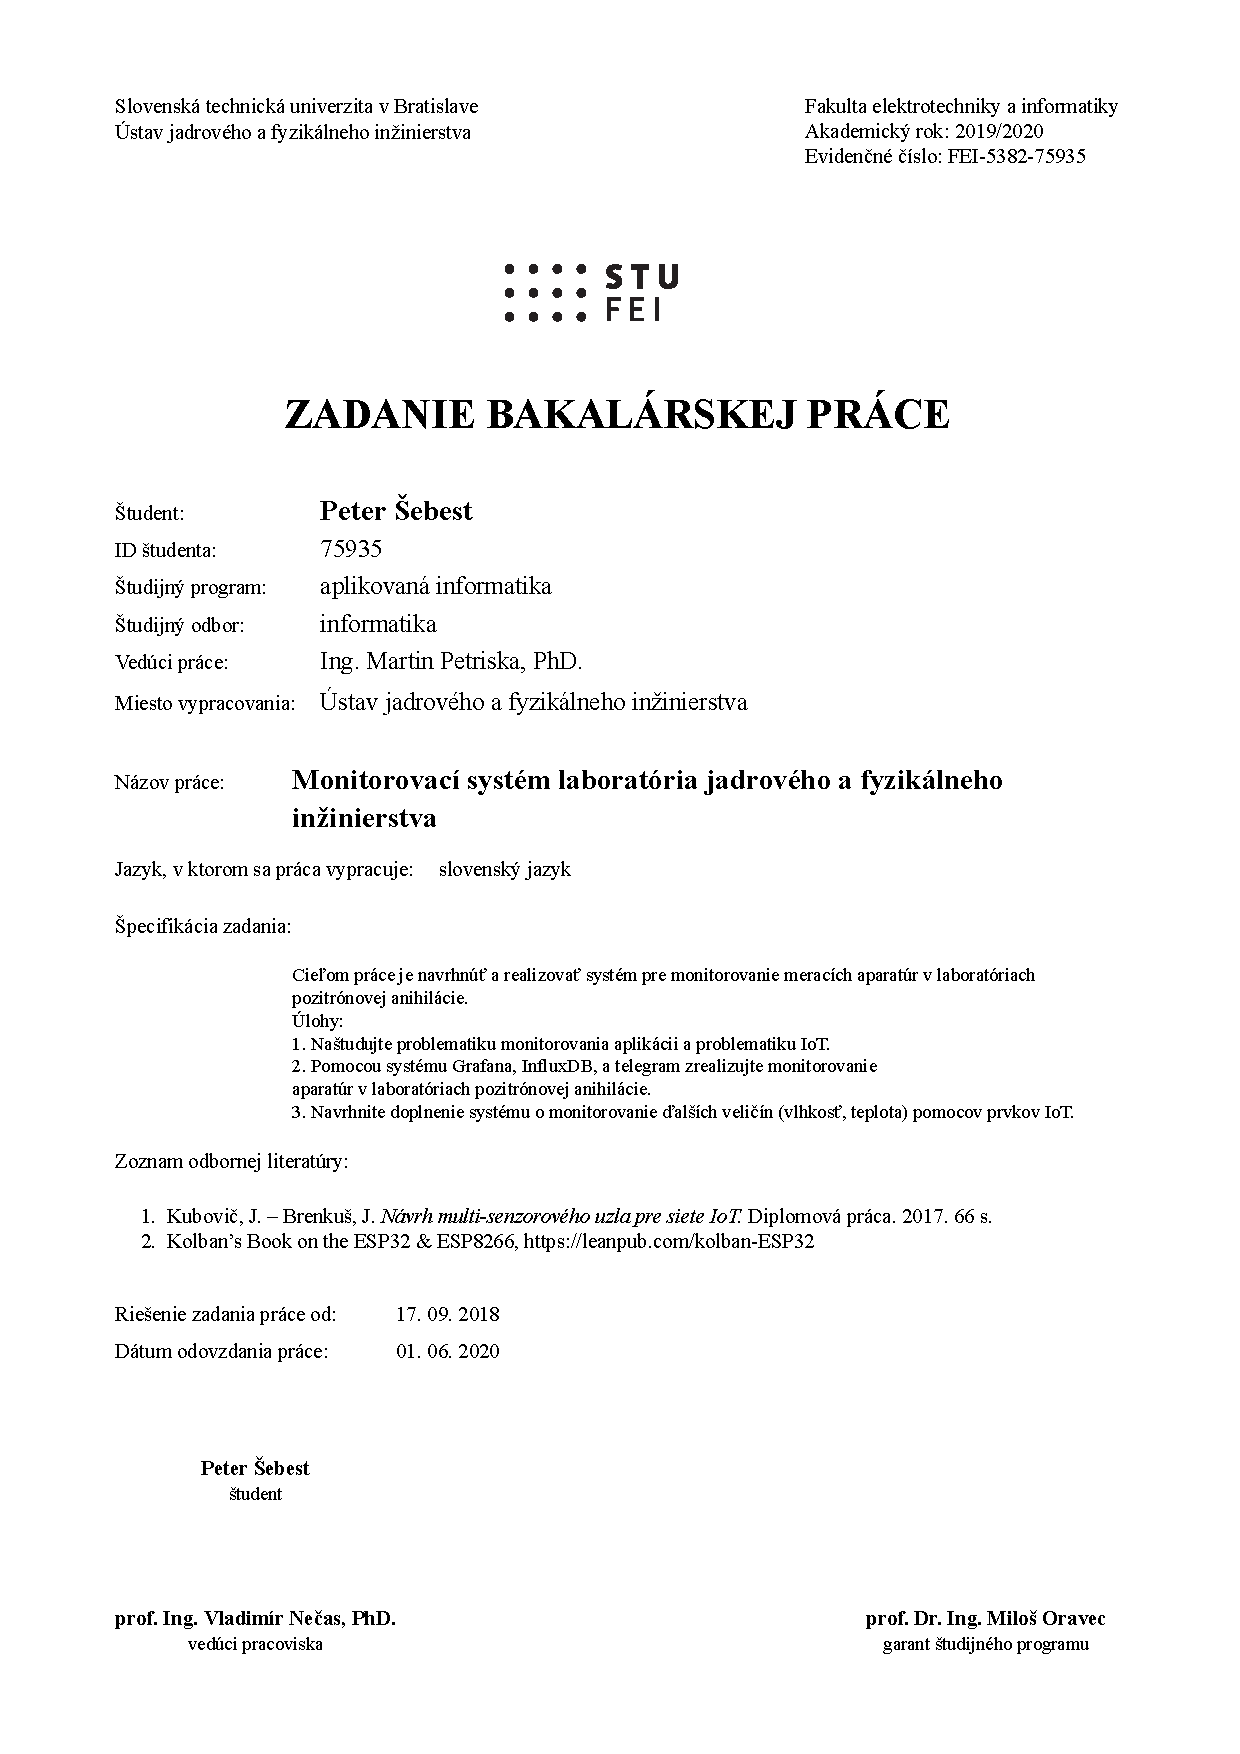
\includepdf[pages=1]{Zadanie.pdf}
%\includepdf[pages=2]{zadanieSebest2.pdf}
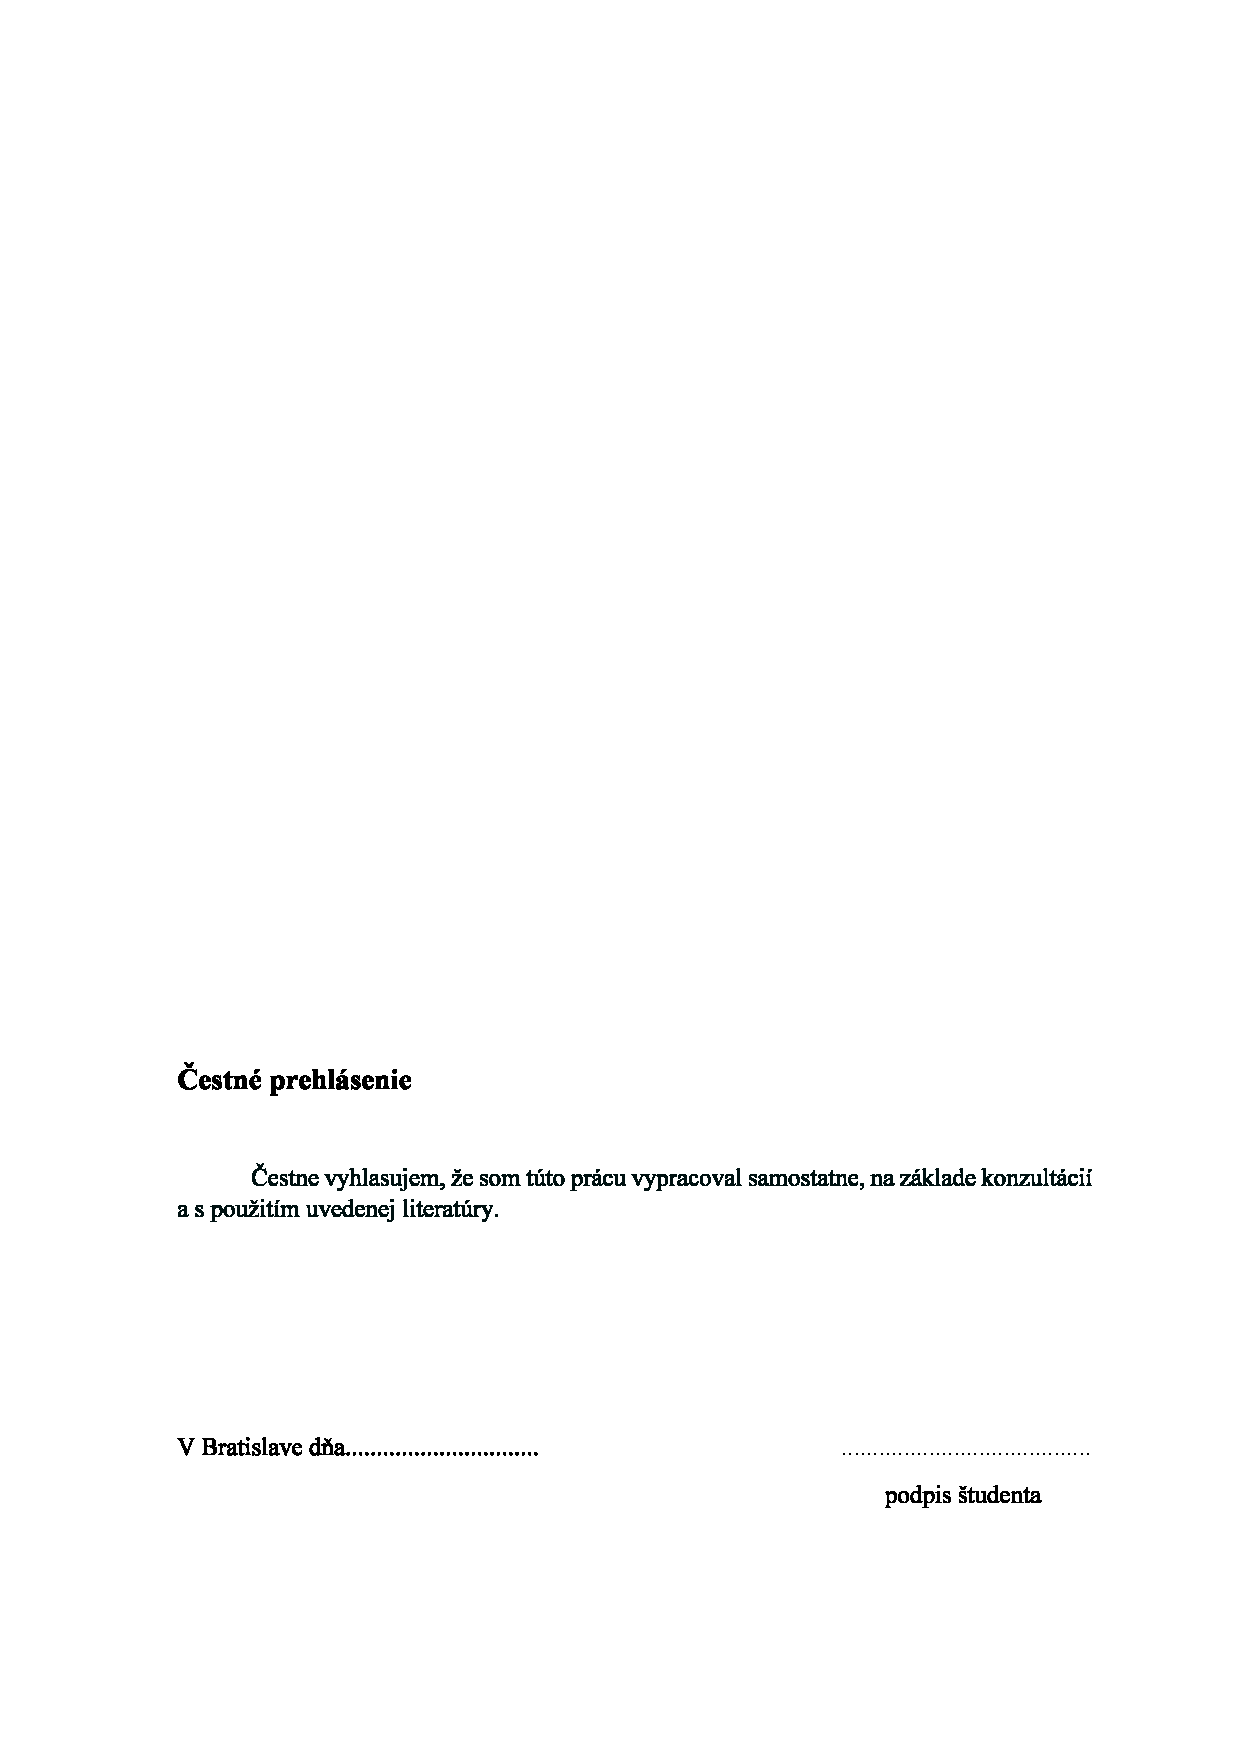
\includepdf[pages=1]{cestne_vyhlasenie.pdf}

\openright

% Struktura prace:
% uvod : zadefinovanie problemu, jeho sucasny stav
% 1 cast:  navrhnutie riesenia - ako to vyriesit
% 2 cast:  ako si to riesil, alebo sme riesili, co sme pouzili
% 3 cast: zhodnotenie toho co sa spravilo ako zodpoveda tomu co sme chceli
% zaver - plan do buducna, ako to vyuzit, co este treba spravit
\loadgeometry{g}

\subfile{uvodna_cast/anotacia.tex}
\subfile{uvodna_cast/abstraktEN.tex}

\newpage

\subfile{uvodna_cast/podakovanie.tex}

\subfile{uvodna_cast/uvod.tex}

\begin{flushleft}
\tableofcontents
\end{flushleft}


\newpage

% \noindent
% \mainmatter
\section{Technológie}
\subfile{./sections/IOT/IOT_main.tex}
\subfile{./sections/Cloud_computing/Cloud_computing_main}
\subfile{./sections/docker/docker_main}
\subfile{./sections/grafana/grafana_main.tex}
\subfile{./sections/influx_DB/influx_main}
\subfile{./sections/node_red/node_red_main}
\subfile{./sections/esp32/Esp32_main.tex}
\subfile{./sections/others/radioaktivita.tex}

\newpage
\section{Implementácia}
\subfile{./implementacia/planovane_riesenie.tex}
\subfile{./implementacia/local.tex}
\subfile{./implementacia/docker_on_azure.tex}
\subfile{./implementacia/meranie.tex}

% Zaverecna cast

\subfile{zaverecna_cast/zaver.tex}
\subfile{zaverecna_cast/images_tables.tex}

\bibliographystyle{unsrt}
\bibliography{literatura}



% \listoffigures

% \pagestyle{plain}
% \setcounter{page}{1}


% \restoregeometry% used with new geometry

\end{document}
